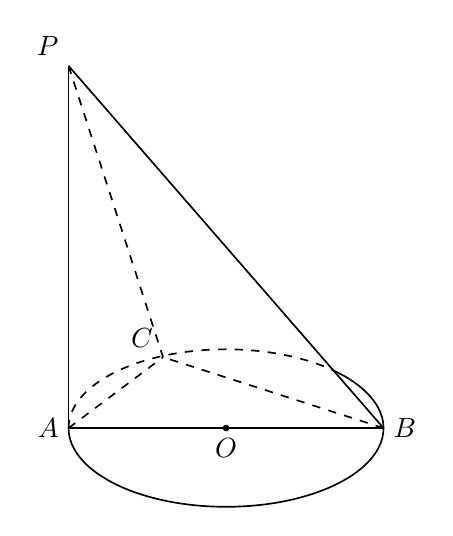
\begin{tikzpicture}[line width=.6pt, font=\normalsize]
  \coordinate (P) at (0,5.2);
  \coordinate (A) at (0,0.6);
  \coordinate (B) at (4,0.6);
  \coordinate (O) at (2,0.6);
  \coordinate (C) at (1.2,1.5);
  % base ellipse: front solid, back dashed
  \draw (0,0.6) arc (180:360:2 and 1);
  \draw[dashed] (0,0.6) arc (180:46.9971313519:2 and 1);
\draw ({2+2*cos(46.9971313519)},{0.6+sin(46.9971313519)}) arc (46.9971313519:0:2 and 1);
  % diameter AB
  \draw (A) -- (B);
  \fill (O) circle (1.2pt);
  \node[below] at (O) {$O$};
  % vertical edge PA and slant PB
  \draw (P) -- (A);
  \draw (P) -- (B);
  % interior dashed edges PC, AC, BC
  \draw[dashed] (P) -- (C);
  \draw[dashed] (A) -- (C);
  \draw[dashed] (B) -- (C);
  \node[above left] at (P) {$P$};
  \node[left] at (A) {$A$};
  \node[right] at (B) {$B$};
  \node[above left] at (C) {$C$};
\end{tikzpicture}
